

\documentclass[oneside]{book}

%\usepackage[utf8]{inputenc}
%\usepackage[english]{babel}
%\usepackage{biblatex}

\usepackage[backend=biber]{biblatex}


\def \CourseName {انتقال داده‌ها}
\def \Instructor {ابولفضل دیانت}
\def \Student {محمدحسین حسنی - ملیکا محمدی فخار}
\def \Semester {نیم‌سال اول\\سال تحصیلی ۱۴۰۳-۱۴۰۲}
\def \PickedSubject {اضافه و حذف کردن نویز به تصویر}
\usepackage[]{algorithm2e}
\usepackage{calc}
\usepackage{fancyhdr}
\usepackage{lipsum}
\usepackage{suffix}
\usepackage{color}
\usepackage[usenames,dvipsnames]{xcolor}
\usepackage[breakable, theorems, skins]{tcolorbox}
\usepackage{ragged2e}
\usepackage[inline]{enumitem}
\usepackage[dvipsnames]{xcolor}
\usepackage{graphicx}
\usepackage{wrapfig}
\usepackage{float}
\usepackage{import}
\usepackage{biblatex}
\usepackage[skip=12pt,indent=2em]{parskip}
\usepackage{setspace}
\usepackage{textcomp}
\usepackage{etoolbox}
\usepackage{xpatch}
\usepackage{footmisc}
\usepackage{longtable} 
\usepackage{todonotes}

\usepackage{tabu}
\usepackage{hyperref}

\usepackage[linewidth=1.5pt,linecolor=red]{mdframed}
\hypersetup{
    colorlinks=false,
    citecolor=black,
    filecolor=black,
    linkcolor=black,
    urlcolor=black
}
\tcbset{enhanced}


\usepackage{listings}
\usepackage{color} %red, green, blue, yellow, cyan, magenta, black, white
\definecolor{mygreen}{RGB}{28,172,0} % color values Red, Green, Blue
\definecolor{mylilas}{RGB}{170,55,241}






\usepackage{minted}
\graphicspath{{images/}{../images/}}
\usepackage{subfiles} 
\usepackage{xepersian} 
\settextfont[Path=./fonts/,
BoldFont={XB Yas Bd}, 
ItalicFont={XB Yas It},
BoldItalicFont={XB Yas BdIt},
Extension = .ttf]{XB Yas}

%---------------------------------define color-------------------------------
\definecolor{gray}{rgb}{0.4,0.4,0.4}
\definecolor{dkgreen}{rgb}{0,0.6,0}
\definecolor{gray}{rgb}{0.4,0.4,0.4}
\definecolor{mauve}{rgb}{0.58,0,0.82}
\definecolor{mygray}{rgb}{0.9,0.9,0.9}
\definecolor{myCyan}{rgb}{0,1,1}
\definecolor{navyBlue}{HTML}{0a065d}
\definecolor{aliceblue}{rgb}{0.94, 0.97, 1.0}
%----------------------------------------------------------------------------


\setminted{
    frame=none,
    framesep=2mm,
    baselinestretch=1.0,
    xrightmargin=0in,
    xleftmargin=0in,
    fontsize=\footnotesize,
    bgcolor=aliceblue,
    linenos=true
}

\makeatletter
\renewcommand{\todo}[2][]{%
    \@todo[caption={\rl{#2}}, #1]{\begin{spacing}{0.5}\rl{#2}\end{spacing}}%
} 
\makeatother 


\setcounter{tocdepth}{1}

\hypersetup{
    colorlinks=true,
    linkcolor=blue,
    filecolor=magenta,      
    urlcolor=blue,
}
\setlist[enumerate]{itemsep=-3mm}
\setlist[itemize]{itemsep=-3mm}


\newfloat{program}{thp}{lop}
\floatname{program}{نمونه کد}
\newcommand{\programref}[1]{نمونه کد \ref{#1}}

\renewcommand{\chaptername}{پروژه}
\renewcommand{\baselinestretch}{1.5}
\newcommand{\grayBox}[1]{\colorbox{gray!10}{\lr{\texttt{#1}}}}
\newcommand{\grayLBox}[1]{\fbox{\grayBox{\parbox{11.8 cm}{#1}}}}

\AtBeginEnvironment{minted}{\setlength{\parskip}{-20pt}}
\xpretocmd{\inputminted}{\par\vspace{-10pt}}{}{}
\xapptocmd{\inputminted}{\par\vspace{-20pt}}{}{}


\newcommand\chapterauthor[1]{\authortoc{#1}\printchapterauthor{#1}}

\makeatletter
\newcommand{\printchapterauthor}[1]{%
    {\parindent0pt\vspace*{-25pt}%
        \linespread{1.1}\large\scshape#1%
        \par\nobreak\vspace*{35pt}}
    \@afterheading%
}
\newcommand{\authortoc}[1]{%
    \addtocontents{toc}{\vskip-10pt}%
    \addtocontents{toc}{%
        \protect\contentsline{chapter}%
        {\hskip1.3em\mdseries\scshape\protect\scriptsize#1}{}{}}
    \addtocontents{toc}{\vskip5pt}%
}
\makeatother


\let\originalinputminted\inputminted
\renewcommand{\inputminted}[2]{
    \originalinputminted[frame=none]{#1}{S\Session/#2}
}


\DeclareRobustCommand{\mybox}[2][gray!20]{%
    \begin{tcolorbox}[   %% Adjust the following parameters at will.
        breakable,
        left=0pt,
        right=0pt,
        top=0pt,
        bottom=0pt,
        colback=#1,
        colframe=#1,
        width=\dimexpr\textwidth\relax, 
        enlarge left by=0mm,
        boxsep=5pt,
        arc=0pt,outer arc=0pt,
        ]
        #2
    \end{tcolorbox}
}
\title{
    \center
    
\includegraphics[width=5cm, height=5cm]{images/IUST_logo_color.png} \\

\CourseName \\[20pt]

موضوع پروژه : 
\PickedSubject  \\
}

\author{
    \textbf{استاد درس:}
    \Instructor \\[10pt]
    \textbf{نام دانشجو:}
    \Student \\[10pt]
}

\date{\Semester}






\begin{document}

\lstset{language=Matlab,%
    %basicstyle=\color{red},
    breaklines=true,%
    morekeywords={matlab2tikz},
    keywordstyle=\color{blue},%
    morekeywords=[2]{1}, keywordstyle=[2]{\color{black}},
    identifierstyle=\color{black},%
    stringstyle=\color{mylilas},
    commentstyle=\color{mygreen},%
    showstringspaces=false,%without this there will be a symbol in the places where there is a space
    numbers=left,%
    numberstyle={\tiny \color{black}},% size of the numbers
    numbersep=9pt, % this defines how far the numbers are from the text
    emph=[1]{for,end,break},emphstyle=[1]\color{red}, %some words to emphasise
    %emph=[2]{word1,word2}, emphstyle=[2]{style},    
}

\pagenumbering{gobble}
\pagestyle{headings}
\maketitle
\pagenumbering{arabic}



\def \Subject {سیگنال تصویر و اضافه کردن نویز}
\def \Author {محمدحسین حسنی - ملیکا محمدی فخار}

\section{گام اول}
با توجه به این که حجم برنامه matlab به شدت بالاست (حدود ۱۸ گیگابایت) از کامپایلر آنلاین octave-online استفاده کردیم.
\section{گام دوم}
در این گام عکسی را به عنوان ورودی برنامه‌مان انتخاب می‌کنیم
.
\begin{figure}[H]
    \centering
    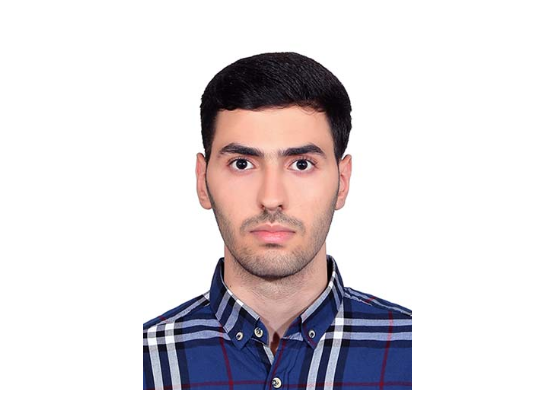
\includegraphics[width=0.65\linewidth]{images/first.png}
    \caption{عکس ورودی}
    \label{fig:h}
\end{figure}
\subsection{بررسی کد}
حال کد متلب این گام را بررسی می‌کنیم
:

\lr{\lstinputlisting{MatlabCode/step1.m}}

حال به بررسی خطوط کد می‌پردازیم:
\begin{itemize}
    \item اول مسیر فایل داده‌شده را مشخص میکنیم
    \item سپس با دستور 
    \(imread\)
     آن فایل را می‌خوانیم
    \item
    و با دستور
    \(imshow\)
    فایل مرحله قبل را در خروجی نشان می‌دهیم.
\end{itemize}

\section{گام سوم}
در این گام با توجه به راهنمایی گفته شده در داک پروژه از تابع پیش تعریف‌شده 
\grayBox{
\(rgb2gray\)
}
استفاده می‌کنیم.
\\
\\
\subsection{بررسی کد}
حال کد متلب این گام را بررسی می‌کنیم
:
\lr{\lstinputlisting{MatlabCode/step3.m}}

\subsection{انواع تصاویر}
\begin{itemize}
    \item 
    \grayBox{binary images }
    : 
    این نوع تصاویر در یک ماتریس 
    \(m * n\)
    ذخیره می‌شوند که رنگ سیاه در آن معادل صفر و رنگ سفید معادل یک می‌باشد
    
    \item
    \grayBox{grayscale images }
     : 
    در
    این نوع تصاویر
    که در یک ماتریس
        \(m * n\)
ذخیره می‌شوند
    هر عضو آن شدت رنگ آن پیکسل را نشان می‌دهد.
   که بزرگترین عدد برای رنگ سفید و کوچکترین عدد برای رنگ سیاه می‌باشد 
   که با توجه به تایپ داده ها می‌توانند رنج مختلفی برای خود بگیرند 
   \item \grayBox{truecolor images(rgb images)}
   : 
   این نوع تصاویر در یک ماتریس سه بعدی یعنی 
       \(m * n * 3\)
       ذخیره می شوند که به جای ذخیره کردن عدد در مرحله قبل یک ماتریس ۳ عضوی 
       متشکل از شدت رنگ های
       rgb
       را در خود نگه می دارد.

\end{itemize}
\section{گام چهارم}
تصویر تبدیل‌شده در مرحله قبل را در نشان داده و آن را ذخیره می‌کنیم.
\subsection{بررسی کد}
\lr{\lstinputlisting{MatlabCode/step4.m}}
\begin{figure}[H]
    \centering
    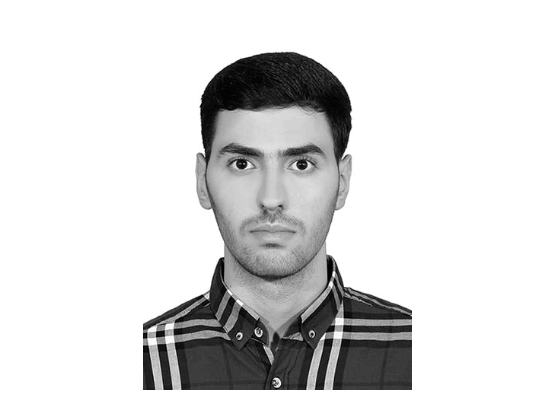
\includegraphics[width=0.65\linewidth]{images/gray.png}
    \caption{تصویر خاکستری‌شده  }
    \label{fig:h}
\end{figure}

\subsection{تفاوت فرمت های متفاوت عکس}
\begin{itemize}
    \item \grayBox{jpg}
    :
    این نوع تصاویر از نوع 
    فشرده‌سازی با اتلاف
    \footnote{compression lossy }
    می‌باشند.
    در 
    واقع حجم فایل را تا حد زیادی کاهش می‌دهد
    این نوع داده برای نگه‌داری و فرستادن مناسب است
    \item \grayBox{png}
    :
    این نوع تصایر از نوع فشرده‌سازی 
    بدون اتلاف
    \footnote{ compression lossless}
    می‌باشند.
    در واقع این نوع فشرده‌سازی مخالف فشرده‌سازی قبلی می‌باشد و می‌توان به بازسازی دوباره داده اصلی از فایل فشرده رسید.
    \item \grayBox{bmp}
    :
    توسط شرکت 
    Microsoft   
    توسعه یافته‌شده است.
    حجم فایل بیشتری دارد
    و از نوع 
    فشرده‌سازی بدون اتلاف می‌باشد.
    \item \grayBox{tiff}
    :
    این نوع نسبت به نوع های‌های قبل بیشترین حجم فایل را دارد و از نوع 
    فشرده‌سازی بدون اتلاف می‌باشد و معمولا در صنعت هنور و عکس‌های حرفه‌ای استفاده می‌شود
\end{itemize}

\textbf{اگر بخواهیم از بین این فرمت ها یک فرمت را به عنوان فشرده‌سازی بدون اتلاف انتخاب کنیم کدام فرمت می‌باشد؟}
\grayBox{.tiff}
\section{گام پنجم}
با توجه به جستجوهای صورت‌گرفته تصویرها از نوع سیگنال توان نیستند اما از نوع سیگنال انرژی می‌باشند.
در پی جستجوهای مختلف 
متوجه شدیم هر عضو ماتریس نشان‌دهنده انرژی آن می‌باشد که با جمع آن‌ها می‌توان به انرژی کل تصویر رسید.
دو راه را برای این‌کار انجام دادیم یکی که طبق نکته ذکرشده بالا و دیگری 
طبق رابطه پارسوال اول تبدیل فوریه آن را محاسبه کرده و سپس انرژی این سینگال را در حوزه فرکانس حساب می‌کنیم.

\subsection{بررسی کد}
\lr{\lstinputlisting{MatlabCode/step5.m}}
\grayLBox{
    totalEnergy : 28313081,
    energy : 1027740529051912
}
\\
\section{گام ششم}
در این گام نیز با توجه به تابع از پیش تعریف‌شده
\grayBox{
    \(imnoise\)
}
که مقادیر پیش‌فرضمقادیر 
 \(0.01\)
برای واریانس و صفر برای میانگین در نظر گرفته‌شده است می‌توان به تصویر نویز اضافه کرد.
و به عنوان ورودی دوم تابع نویز
\grayBox{\(gaussian\)}
را به آن می‌دهیم
و در ادامه نویز اضافه شده به تصویر را نمایش می‌دهیم.
\subsection{بررسی کد}
\lr{\lstinputlisting{MatlabCode/step6.m}}
\begin{figure}[H]
    \centering
    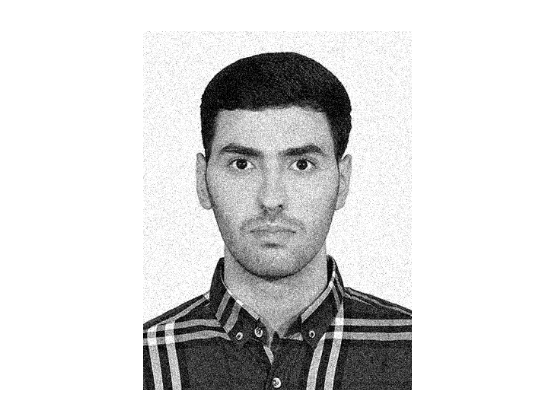
\includegraphics[width=0.65\linewidth]{images/noisy.png}
    \caption{ تصویر با نویز }
    \label{fig:h}
\end{figure}

\subsection{\lr{SNR(signal to noise ratio)}}
در این قسمت نوبت به محاسبه نسبت سینگال به نویز اضافه شده‌است. 
\\
\grayBox{SNR}
:
میزان قدرت یک سیگنال نسبت به نویز پس‌زمینه آن می‌باشد.
که با با واحد 
\(db\)
اندازه‌گیری می‌شود.
\null \hfill $ SNR =  10 \cdot \log_{10} \dfrac{P_{signal}}{P_{noise}}$

این نسبت می‌تواند هر عددی باشد که اعداد بزرگتر از صفر نشان دهنده این است که سطح سیگنال اصلی بیشتر از سطح noise است 
و اعداد کوچکتر برعکس. 
در واقع هر چه این نسبت بزرگتر باشد کیفیت سیگنال بهتر است.

\subsection{بررسی کد}
\lr{\lstinputlisting{MatlabCode/snr.m}}
\grayLBox{signalNoiseRatio = 14.59}


\section{گام هفتم}
در این گام سعی به گرفتن تبدیل فوریه از تصویر خاکستری شده و آن را طبق راهنمایی گفته شده رسم می‌کنیم.
\\
\subsection{بررسی کد}
\lr{\lstinputlisting{MatlabCode/step7.m}}

\begin{figure}[H]
    \centering
    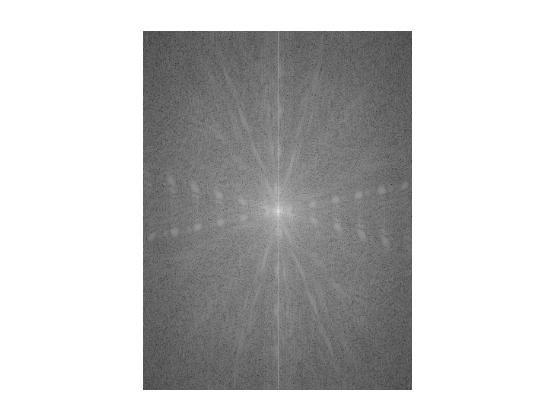
\includegraphics[width=0.65\linewidth]{images/fourier.png}
    \caption{ تصویر تبدیل فوریه گرفته شده }
    \label{fig:h}
\end{figure}

\subsection{تحلیل تبدیل فوریه گرفته شده}

\begin{itemize}
    \item هر پیکسل در عکس تبدیل فوریه نشان دهنده 
    یک موج سینوسی دو بعدی با فرکانس وابسته به فاصله از مرکز می‌باشد.
    \item نتیجه تصویر نشان می‌دهد که عکس حاوی تمامی فرکانس‌ها می‌باشد اما بزرگی آن هر چه از مرکز تصویر دورتر می‌شویم کمتر می‌شود و در نتیجه فرکانس بیشتر می‌شود.
    \item 
    فرکانس‌های کمتر حاوی اطلاعات بیشتری نسبت به فرکانس های بالاتر هستند
\end{itemize}
\subsection{پاسخ به سوال‌ها}
\begin{enumerate}
    \item \textbf{مرکز تصویر چرا از همه نقاط دیگر نورانی تر است؟}
    به دلیل اینکه بخش زیادی از عکس فرکانس کمتری دارند و مرکز تصویر حاوی اطلاعات بیشتری است.
    به تعبیری دیگر بخش زیادی از تصویر اصلی ما داری تغییرات کم فرکانس هستند یعنی رنگ آنها به یک‌باره از سفید به سیاه تغییر نمی‌کند
    \item \textbf{چرا هر چه از مرکز دورتر می‌شویم نقاط کم نورتر می شوند؟}
    چون این نقاط فرکانس بیشتر را در بر می‌گیرند در واقع این نفاط نشان‌دهنده تغییر ناگهانی در عکس اصلی می‌باشند.
    \item \textbf{بالا و پایین‌ترین فرکانس در تصویر کدام نقاط است؟}
    مرکز دارای کمترین فرکانس و هرچه از مرکز دورتر می‌شویم فرکانس بیشتر می‌شود.
\end{enumerate}
\section{گام هشتم}
از روش 
\grayBox{\(median\)}
استفاده می‌کنیم.
\subsection{بررسی کد}
\lr{\lstinputlisting{MatlabCode/step8.m}}

\begin{figure}[H]
    \centering
    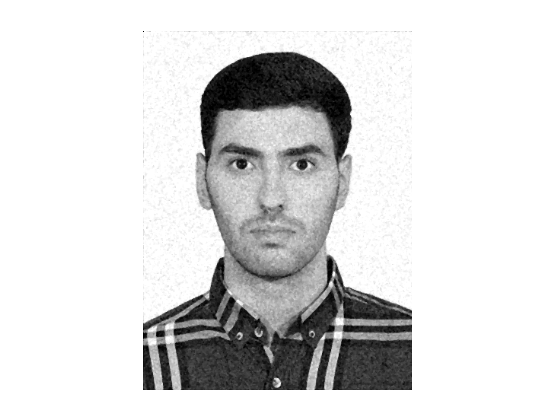
\includegraphics[width=0.65\linewidth]{images/removednoise.png}
    \caption{ تصویر با نویز رفع‌شده }
    \label{fig:h}
\end{figure}

\subsection{عملکرد رفع نویز }
با توجه به راهنمایی گفته‌شده و تابع ازپیش‌تعریف‌شده 
\grayBox{\(PSNR\)}
به بررسی این تابع می‌پردازیم
.
هرچه مقدار خروجی این تابع بیشتر باشد ما بهتر عمل کرده‌ایم
\subsubsection{PSNR range}
\begin{itemize}
    \item برای تصویر ها و ویدئو های فشرده شده بین 
    ۳۰ تا ۵۰ دسی‌بل می‌باشد
    که ۸ بیتی است.
    \item برای ۱۲ بیتی خروجی از ۶۰ به بالا خوب است
    \item مقدارهای قابل‌قبول برای انتقال‌های بی‌سیم بین ۲۰ تا ۲۵ می‌باشد.
\end{itemize}
\lr{\lstinputlisting{MatlabCode/peakSNR.m}}
\grayLBox{The Peak-SNR value is 18.3259}



\nocite{*}

\end{document}
